% Background (lay out the details of the problem setting)
\section{Background}

As my personal research is in the field of formal synthesis and GI, I would like to focus on more popular, deep learning-based methodolgies from the broad \textbf{field of learning from demonstrations (LfD)}, which will make an excellent comparison study for my existing research. There are many, many different ways to approach LfD \cite{Ravichandar2020}, as can be seen in Fig. \ref{fig: lfd_venn}, but two of the most salient and foundational are Maximum Entropy Deep Inverse Reinforcement Learning (MEDIRL) \cite{Wulfmeier2015MaximumED} and Generative Adversarial Imitation Learning (GAIL) \cite{Ho2016GenerativeAI}.

\begin{figure}[htbp]
\centerline{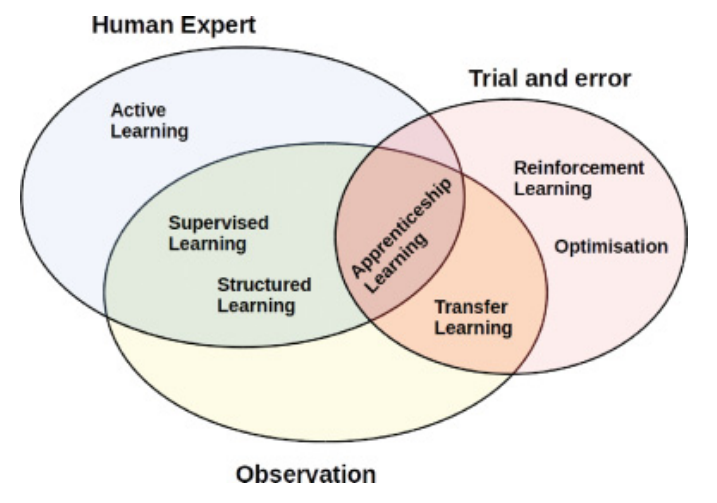
\includegraphics[width=\linewidth]{Figures/lfd_venn_diagram.png}}
\caption{How all the different forms of LfD are interconnected. Reproduced from \cite{Hussein2017}}
\label{fig: lfd_venn}
\end{figure}

MEDIRL proposes using expert trajectories to recover an estimate for the reward function, which it then uses to run reinforcement learning algorithms on to recover a policy. The interesting thing to note here is that the "maximum entropy" term comes from the need to disambiguate the set of reward functions that match the observed trajectories \cite{Wulfmeier2015MaximumED}. In the case of IRL, there are an infinite number of such reward functions, so the novel heuristic here is to choose from those that produce the most entropy. The reward function that induces the most information theoretic policy entropy is likely a good, generalizable reward function as it is the least trivial (from the definition of entropy). This stems from the observation that reward functions that encode complex tasks are rarely trivially definable and sparse, and thus the best choice for a reward function is reward function that applies reward and cost to a large swatch of the state-space \cite{Hussein2017}.

One observation of the observations made in the GAIL paper is that MEDIRL is typically inefficient; most of the time we don't really care about the reward function as only care about learning a controller (policy) for the system. To address this, the authors here suggest a beautiful, if very mathematically intricate, proof that MEDIRL is the dual of the direct occupancy measure matching matching problem (of which they prove all IRL is a subclass of) \cite{Ho2016GenerativeAI}. The occupancy measure for a policy defined on a finite state / action space is essentially the distribution of state-action pairs that an agent encounters when interacting with the environment according to the policy. Although not explicitly explained, they this assumption they can make this assumption without loss of generality \cite{Ho2016GenerativeAI}.

This occupancy re-framing of the IRL problem leads to the conclusion that the primal to the MEDIRL dual optimization problem is indeed recovering a policy that directly matches the observed expert's problem occupancy measure. With this in mind, the GAIL algorithm is essentially trying to minimize an entropy-constrained occupancy cost regulizer and the entropy of the learned policy. The authors saw the connection between this algorithm and that of generative adversarial neural network architectures (GANs), where a generator network tries to produce examples that fool an adversarial classification network. This unsupervised learning algorithm is exactly the same as the imitation learning algorithm, where the "generator" is the policy network being trained by policy gradient from a reward signal given by the "adversarial" classifier that is trained to distinguish real state-action pairs sampled from the expert from state-action pairs sampled from the policy network \cite{Ho2016GenerativeAI}.

What this amounts to is basically building two neural networks, one that classifies policies as either learned or from the expert, and one standard policy network. The classifier is trained based with a standard classification loss, which is turned into a "reward" signal that the policy network network can use to train with RL. Thus, the policy network never actually interacts with the environment, but you can still use standard policy gradient methods as the basic RL algorithm (e.g. TRPO, PPO2). 

The very interesting ideas presented in the GAIL framework are very powerful (GANs are really powerful and cool ways to learn a distribution) make it an appealing methodology for exploration in this project on LfD.